\chapter{Theoretischer Hintergrund}
\label{chap:hintergrund}
Um das Verständnis dieser Arbeit zu erleichtern, werden in diesem Kapitel zunächst die für das Quantencomputing relevanten quantenmechanischen Effekte und Notationen sowie die Grundlagen von Quantenschaltkreisen und Quantengattern vermittelt.

% ----------------------------------------------------------------
\section{Superposition}
\label{sec:superposition}
Im Gegensatz zum klassischen Bit, das entweder den Wert 0 oder 1 annimmt, bietet das Quantencomputing den Vorteil der Superposition, die durch
Quantenbits, auch Qubits genannt, realisiert wird~\cite{nielsen2010chuang}. Der Zustand eines Qubits ist eine Linearkombination der beiden Basiszustände $\ket{0}$ und
$\ket{1}$ und kann diese vor der Messung gleichzeitig repräsentieren. So spannen $n$ Qubits einen Zustandsraum von $2^n$ Basiszuständen auf. Da eine Messung jedoch nur einen einzelnen Basiszustand liefert, sind diese Zustände nicht direkt auslesbar. Dieses Prinzip bildet eine der fundamentalen Grundlagen des Quantenvorteils gegenüber der klassischen
Datenverarbeitung~\cite{preskill2018quantum}. Dadurch lassen sich Zustände abbilden, die nicht mehr auf $\ket{0}$ und $\ket{1}$ beschränkt sind, wodurch sich Algorithmen entwerfen lassen, die bestimmte Probleme schneller lösen als bekannte klassische Verfahren.
\newpage
\section{Notation von Quantenzuständen}
\label{sec:braket}
Den Zustand eines Qubits beschreibt man sowohl im Quantencomputing als auch in der Quantenmechanik in der sogenannten Dirac-Notation, auch Bra-Ket-Notation genannt. Ein Zustandsvektor wird dabei als Ket $\ket{\psi} = \alpha\ket{0} + \beta\ket{1}$ geschrieben. Hierbei sind $\alpha$ und $\beta$ komplexe Zahlen und werden Amplituden genannt. Es gilt stets die Normierungsbedingung $|\alpha|^2 + |\beta|^2 = 1$, das heißt, die Betragsquadrate ergeben summiert die Wahrscheinlichkeit 1. Wird der Zustand gemessen, so ergibt sich der Wert $0$ mit der Wahrscheinlichkeit $|\alpha|^2$ und der Wert $1$ mit der Wahrscheinlichkeit $|\beta|^2$.
\section{Verschränkung}
\label{sec:verschraenkung}
Ein weiteres fundamentales Phänomen, durch welches sich im Quantencomputing ein Vorteil verschaffen lässt, ist die Verschränkung von Qubits. Bei einem verschränkten reinen Zustand mehrerer Qubits ist der Gesamtzustand mehr als die Summe der einzelnen Zustände. Er lässt sich nicht als Tensorprodukt der Zustände der einzelnen Qubits darstellen~\cite{nielsen2010chuang}. Die einzelnen Qubits besitzen dann keinen eigenen reinen Zustand mehr und können nur noch gemeinsam als zusammenhängendes System vollständig beschrieben werden.
Eine unmittelbare Folge ist, dass die Messergebnisse verschränkter Qubits miteinander korreliert sind. Ein bekanntes Beispiel ist der Bell-Zustand
\[
    \ket{\Phi^{+}} = \frac{1}{\sqrt{2}} \left( \ket{00} + \ket{11} \right),
\]
bei dem die Messung des einen Qubits das Ergebnis des anderen unmittelbar festlegt, obwohl vor der Messung keines der beiden einen definierten Wert besitzt. Diese nicht-klassischen Korrelationen sind eine wesentliche Ressource für viele Quantenalgorithmen und tragen maßgeblich zum Leistungsvorteil gegenüber klassischen Verfahren bei.

\newpage
\section{Bloch-Sphäre}
\label{sec:blochsphaere}
Der Zustand eines einzelnen Qubits lässt sich geometrisch als Punkt auf der Oberfläche einer Einheitskugel darstellen, der sogenannten Bloch-Sphäre~\cite{nielsen2010chuang}. Da eine globale Phase physikalisch nicht messbar ist, genügen zwei reelle Winkel, um den Zustand vollständig zu beschreiben.
\[
    \ket{\psi} = \cos\!\left(\frac{\theta}{2}\right)\ket{0} + e^{i\varphi}\sin\!\left(\frac{\theta}{2}\right)\ket{1}.
\]

\begin{figure}[H]
    \centering
    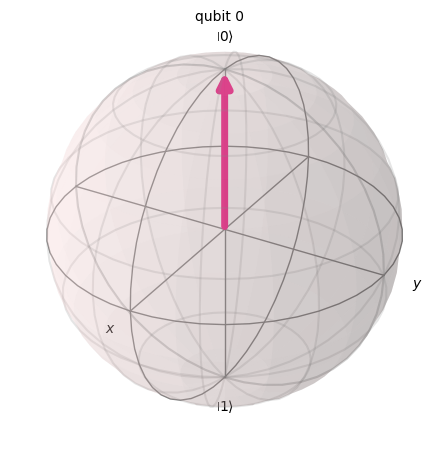
\includegraphics[width=0.5\textwidth]{figures/basis-zustand-blochsphaer.png}
    \caption{Bloch-Sphäre im Basiszustand}
    \label{fig:bloch-basis}
\end{figure}

Der Winkel $\theta$ bestimmt dabei das Verhältnis der beiden Amplituden, der Winkel $\varphi$ ihre relative Phase. Die beiden Basiszustände $\ket{0}$ und $\ket{1}$ liegen am Nord- beziehungsweise Südpol der Kugel, während alle übrigen Punkte der Oberfläche Superpositionen entsprechen. Operationen auf einem Qubit lassen sich in dieser Darstellung als Drehungen des Zustandsvektors um die Achsen der Kugel auffassen. Die Bloch-Sphäre eignet sich damit vor allem zur Veranschaulichung einzelner Qubits.

\newpage
\section{Quantenschaltkreise und Gatter}
\label{sec:gatesCircuits}

Quantenschaltkreise, auch \textit{Circuits} genannt, sind die übliche Darstellungsform für Quantenprogramme im Gattermodell, das auf David Deutsch~\cite{deutsch1985quantum} zurückgeht und heute den Standard für die Programmierung von Quantencomputern bildet. Jedes Qubit erhält seine eigene horizontale Linie, beginnend mit $q_0$.Bei $n$ Qubits hat man daher $n$ Linien, die von $q_0$ bis $q_{n-1}$
nummeriert sind (siehe Abbildung~\ref{fig:circuit-cnot}).. Auf diese Linien werden von links nach rechts \textit{Quantengatter} angewendet, die die Zustände der Qubits manipulieren~\cite{nielsen2010chuang,homeister2022quantum}.
Am Ende eines Circuits steht in der Regel eine \textit{Messung}, die den Quantenzustand auf einen klassischen Bitwert reduziert und pro Qubit den Wert $0$ oder $1$ liefert. Da das Ergebnis einer einzelnen Messung zufällig ist, lässt sich aus einem einzigen Durchlauf noch keine Aussage über den zugrundeliegenden Zustand ableiten. Erst die vielfache Ausführung desselben Circuits liefert eine Verteilung der Ergebnisse, aus der sich die Wahrscheinlichkeiten der möglichen Messwerte abschätzen lassen. Die Anzahl dieser Wiederholungen wird als \textit{Shots} bezeichnet~\cite{nielsen2010chuang,bashiri2025quantencomputing}.

Es gibt verschiedene Arten von Gattern. Einqubit-Gatter lassen sich als $2 \times 2$-Matrix darstellen. Jedoch gibt es auch Gatter, die auf mehrere Qubits wirken. Ein Gatter, das auf $n$ Qubits wirkt, entspricht einer unitären $2^{n} \times 2^{n}$-Matrix.
\newpage

\paragraph*{X-Gatter}\mbox{}\\
Das \textit{X-Gatter} stellt das quantenmechanische Analogon der klassischen
NOT-Operation dar und vertauscht die Amplituden der Basiszustände $\ket{0}$ und
$\ket{1}$. Seine Matrixdarstellung lautet
\begin{equation}
    \mathbf{X} = \begin{pmatrix} 0 & 1 \\ 1 & 0 \end{pmatrix}.
\end{equation}
Angewendet auf den Ausgangszustand $\ket{0}$ ergibt sich
\begin{equation}
    \mathbf{X}\ket{0}
    = \begin{pmatrix} 0 & 1 \\ 1 & 0 \end{pmatrix}
      \begin{pmatrix} 1 \\ 0 \end{pmatrix}
    = \begin{pmatrix} 0 \\ 1 \end{pmatrix}
    = \ket{1}.
\end{equation}
Der Zustand wird somit deterministisch in $\ket{1}$ überführt, es gilt also
$p(0) = 0$ und $p(1) = 1$. Eine Superposition entsteht dabei nicht. Auf der
Bloch-Sphäre entspricht das X-Gatter einer Drehung um $\pi$ um die $x$-Achse,
wodurch der Zustandsvektor vom Nordpol zum Südpol wandert (siehe
Abbildung~\ref{fig:x-gatter}).

\begin{figure}[htbp]
    \centering
    \begin{subfigure}{0.45\textwidth}
        \centering
        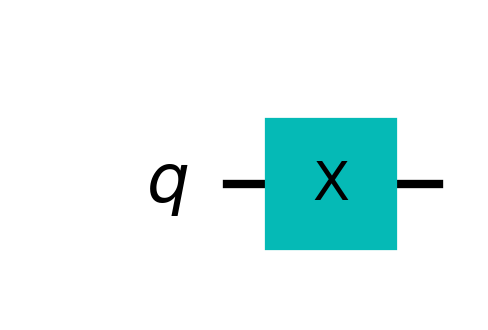
\includegraphics[width=0.65\linewidth]{figures/DarstellungGatter/x_gatter_circuit.png}
        \subcaption{Schaltkreis mit \textit{X}-Gatter}
        \label{fig:circuit-x}
    \end{subfigure}\hfill
    \begin{subfigure}{0.45\textwidth}
        \centering
        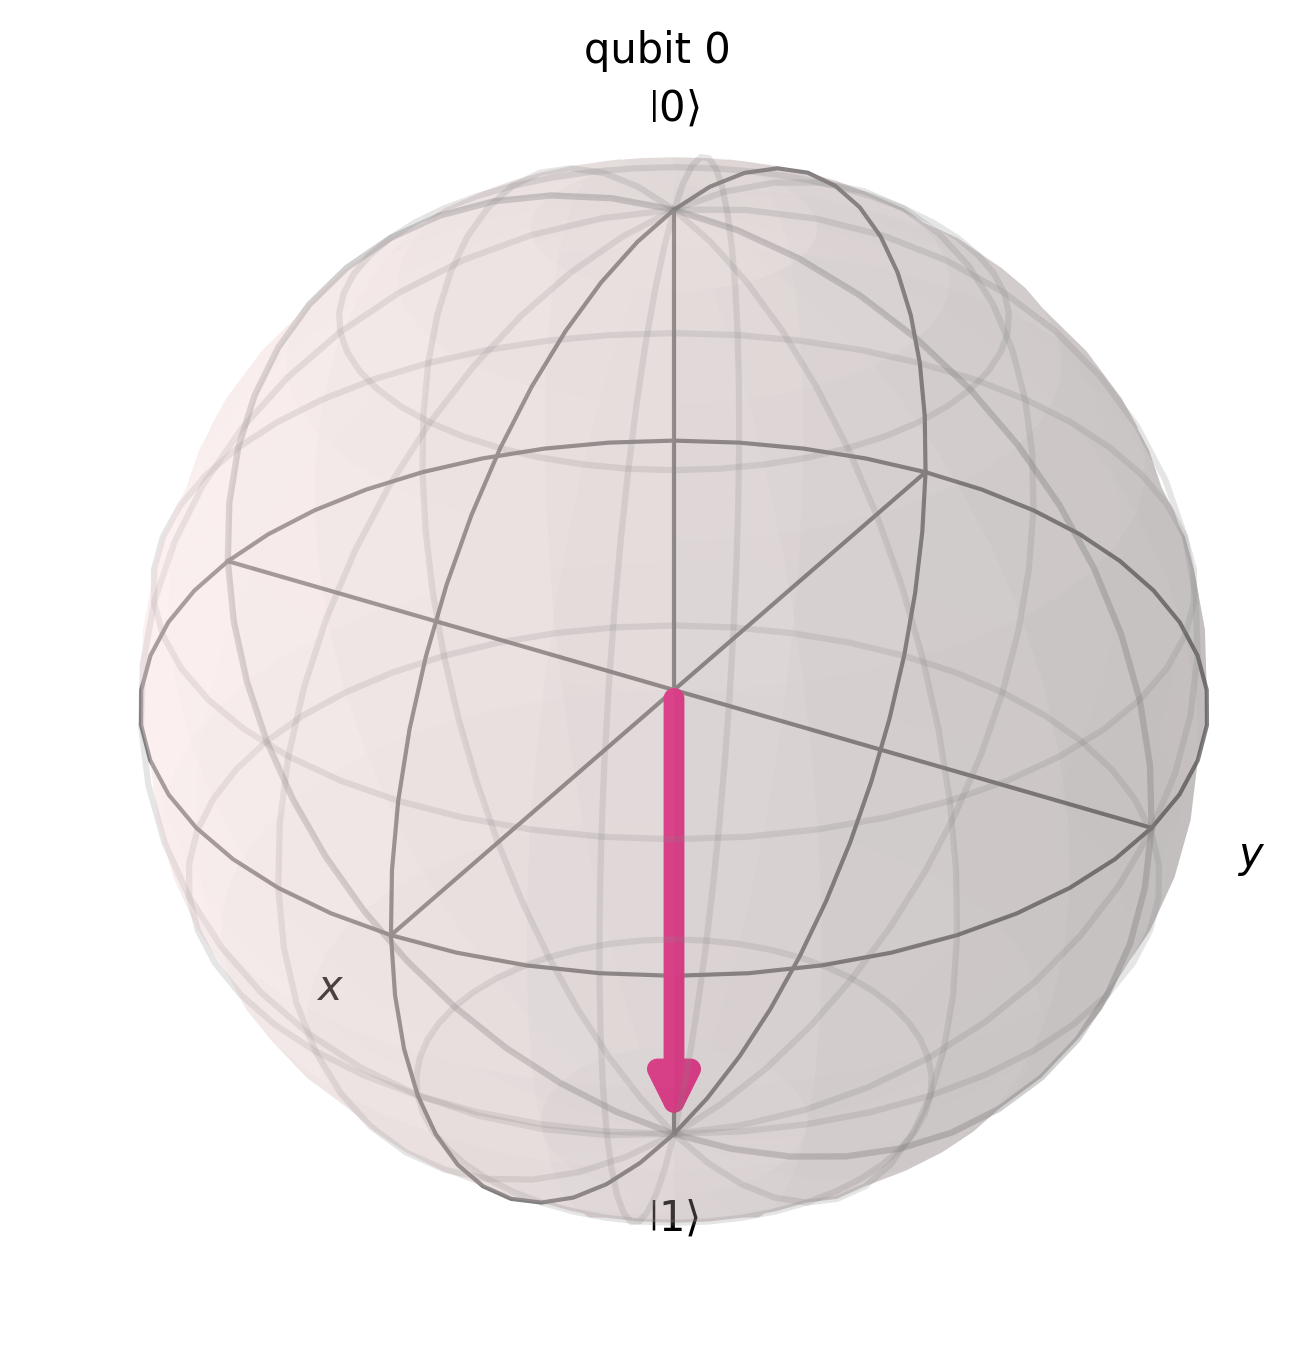
\includegraphics[width=0.65\linewidth]{figures/DarstellungGatter/x_gatter_bloch.png}
        \subcaption{Zustand auf der Bloch-Sphäre}
        \label{fig:bloch-x}
    \end{subfigure}
    \caption{Wirkung des \textit{X}-Gatters}
    \label{fig:x-gatter}
\end{figure}

\paragraph*{Hadamard-Gatter}\mbox{}\\
Das \textit{Hadamard-Gatter} erzeugt aus einem Basiszustand eine gleichgewichtete
Superposition und realisiert damit den Basiswechsel zwischen der $Z$- und der
$X$-Basis. Es besitzt die Matrixdarstellung
\begin{equation}
    \mathbf{H} = \frac{1}{\sqrt{2}}
    \begin{pmatrix} 1 & 1 \\ 1 & -1 \end{pmatrix}.
\end{equation}
Die Anwendung auf den Ausgangszustand $\ket{0}$ liefert
\begin{equation}
    \mathbf{H}\ket{0}
    = \frac{1}{\sqrt{2}}
      \begin{pmatrix} 1 & 1 \\ 1 & -1 \end{pmatrix}
      \begin{pmatrix} 1 \\ 0 \end{pmatrix}
    = \frac{1}{\sqrt{2}}
      \begin{pmatrix} 1 \\ 1 \end{pmatrix}
    = \frac{1}{\sqrt{2}}\bigl(\ket{0} + \ket{1}\bigr).
\end{equation}
Beide Messergebnisse treten folglich mit gleicher Wahrscheinlichkeit
$p(0) = p(1) = \tfrac{1}{2}$ auf, wie in Abbildung~\ref{fig:h-gatter} dargestellt.
Da $\mathbf{H}^2 = \mathbf{I}$ gilt, ist das Hadamard-Gatter zugleich sein eigenes
Inverses.

\begin{figure}[htbp]
    \centering
    \begin{subfigure}{0.45\textwidth}
        \centering
        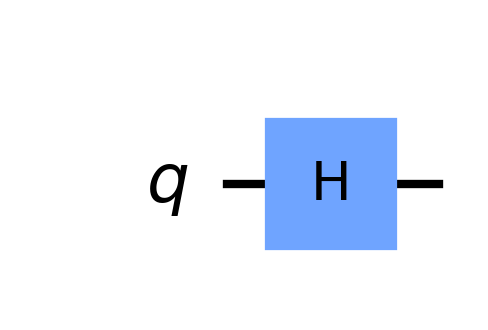
\includegraphics[width=0.65\linewidth]{figures/DarstellungGatter/h_gatter_circuit.png}
        \subcaption{Schaltkreis mit \textit{H}-Gatter}
        \label{fig:circuit-h}
    \end{subfigure}\hfill
    \begin{subfigure}{0.45\textwidth}
        \centering
        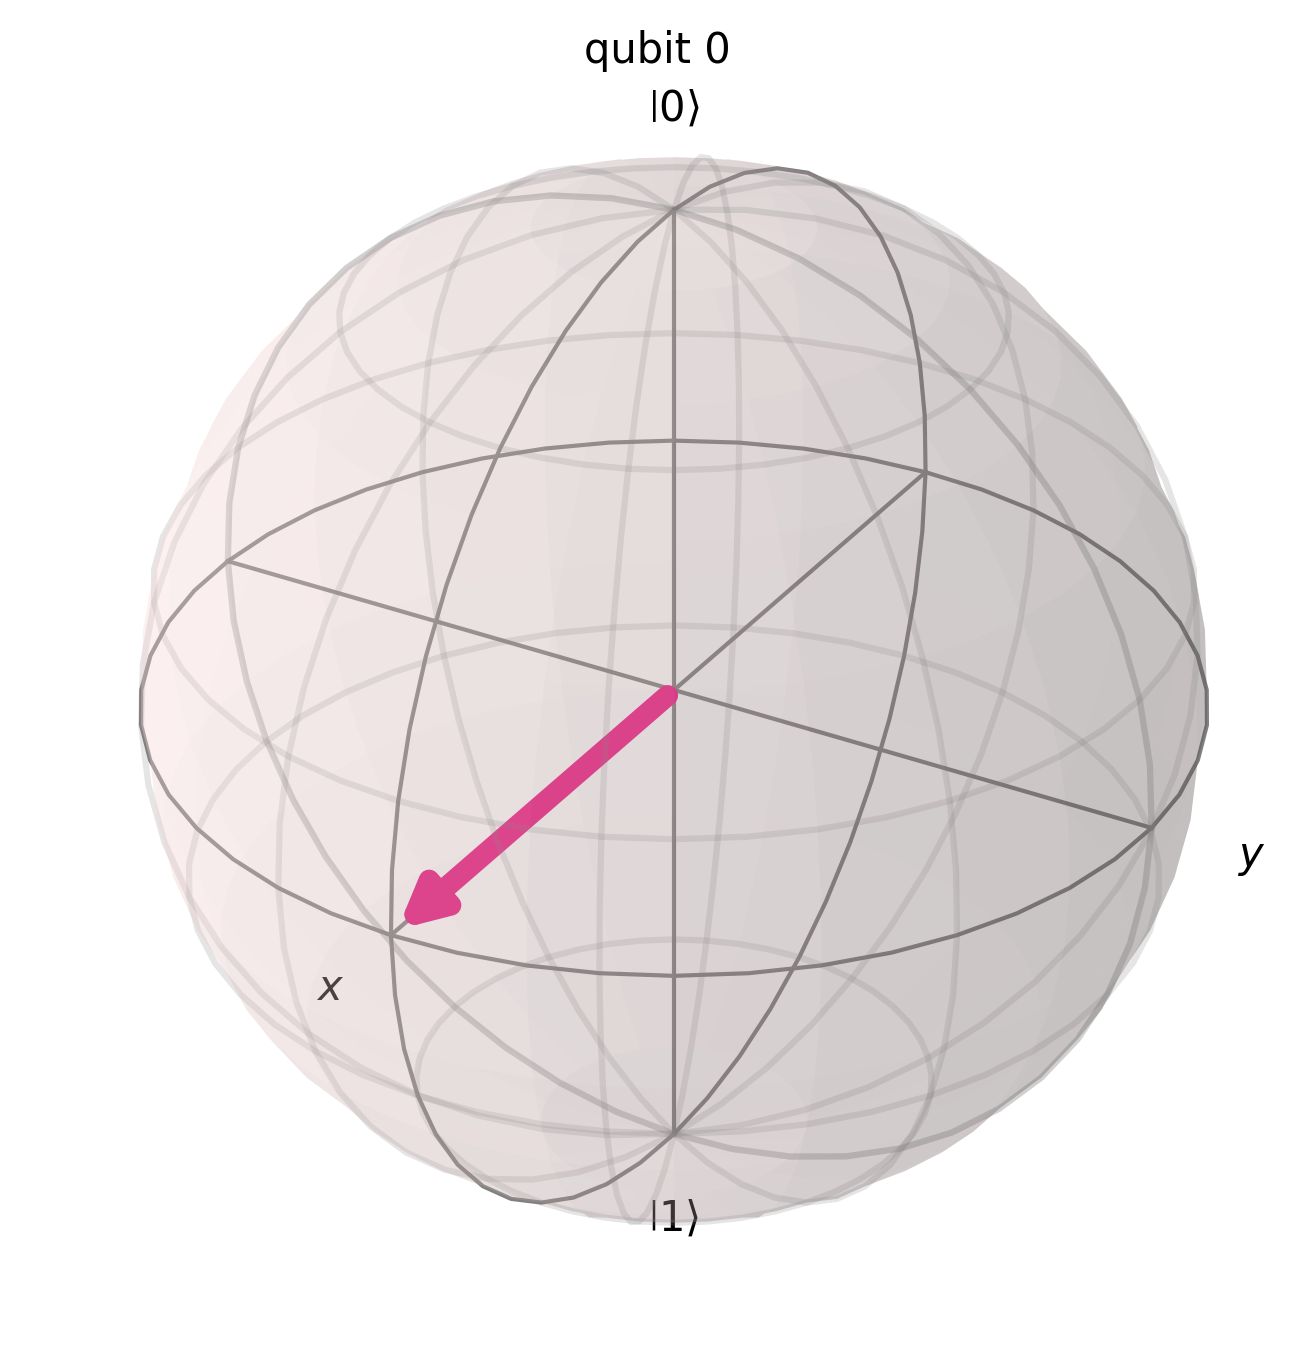
\includegraphics[width=0.65\linewidth]{figures/DarstellungGatter/h_gatter_bloch.png}
        \subcaption{Zustand auf der Bloch-Sphäre}
        \label{fig:bloch-h}
    \end{subfigure}
    \caption{Wirkung des Hadamard-Gatters}
    \label{fig:h-gatter}
\end{figure}

\paragraph*{T-Gatter}\mbox{}\\
Das \textit{T-Gatter} gehört zur Klasse der Phasengatter. Es lässt den Basiszustand
$\ket{0}$ unverändert und prägt dem Zustand $\ket{1}$ eine relative Phase von
$e^{i\pi/4}$ auf. Seine Matrixdarstellung lautet
\begin{equation}
    \mathbf{T} = \begin{pmatrix} 1 & 0 \\ 0 & e^{i\pi/4} \end{pmatrix}.
\end{equation}
Angewendet auf einen allgemeinen Zustand
$\ket{\psi} = \alpha\ket{0} + \beta\ket{1}$ ergibt sich
\begin{equation}
    \mathbf{T}\ket{\psi} = \alpha\ket{0} + e^{i\pi/4}\beta\ket{1}.
\end{equation}
Da die Phase den Betrag der Amplituden nicht verändert, bleiben die
Messwahrscheinlichkeiten in der Rechenbasis unbeeinflusst. Die aufgeprägte
Phaseninformation wird erst durch nachfolgende Gatter beobachtbar, die einen
Basiswechsel bewirken.

Auf den Zustand $\ket{0}$ angewendet, bleibt das T-Gatter ohne Wirkung, da die Phase
allein den Anteil $\ket{1}$ betrifft. Um die Phase überhaupt sichtbar zu machen,
wird dem T-Gatter daher ein Hadamard-Gatter vorangestellt. Dieses erzeugt zunächst
eine gleichgewichtete Superposition, sodass beide Basiszustände am Gesamtzustand
beteiligt sind. Erst dann verschiebt das T-Gatter den Zustandsvektor auf der
Bloch-Sphäre entlang des Äquators um $45$ Grad, wie in
Abbildung~\ref{fig:h-t-gatter} dargestellt. Die Messwahrscheinlichkeiten bleiben
dabei weiterhin bei $p(0) = p(1) = \tfrac{1}{2}$.

\begin{figure}[htbp]
    \centering
    \begin{subfigure}{0.45\textwidth}
        \centering
        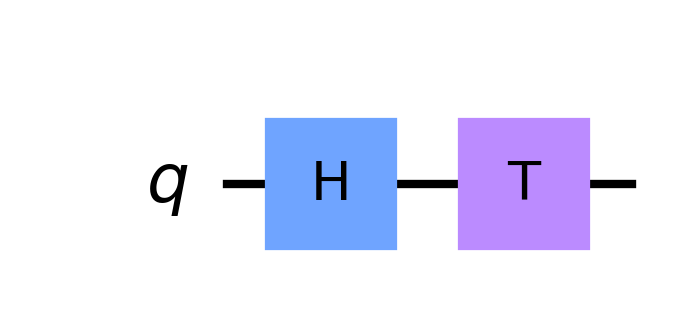
\includegraphics[width=0.65\linewidth]{figures/DarstellungGatter/h_t_gatter_circuit.png}
        \subcaption{Schaltkreis mit \textit{H}- und \textit{T}-Gatter}
        \label{fig:circuit-h-t}
    \end{subfigure}\hfill
    \begin{subfigure}{0.45\textwidth}
        \centering
        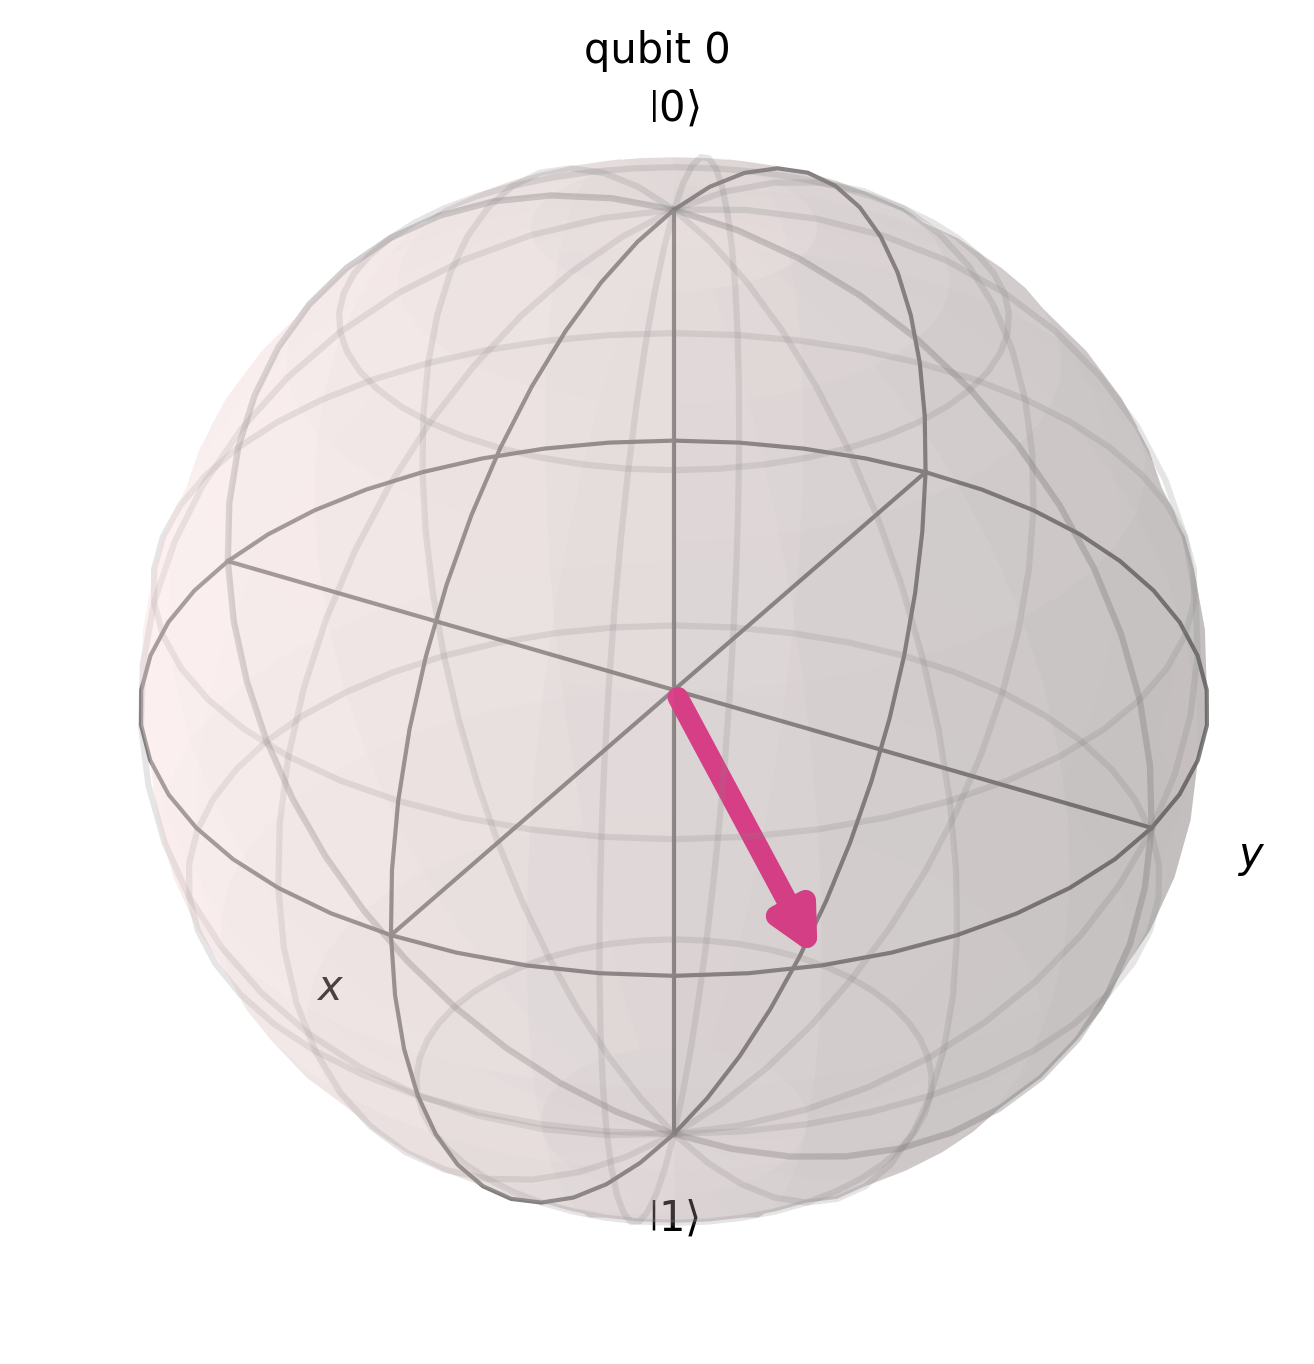
\includegraphics[width=0.65\linewidth]{figures/DarstellungGatter/h_t_gatter_bloch.png}
        \subcaption{Zustand auf der Bloch-Sphäre}
        \label{fig:bloch-h-t}
    \end{subfigure}
    \caption{Sichtbarwerden der Phase durch ein vorgeschaltetes Hadamard-Gatter}
    \label{fig:h-t-gatter}
\end{figure}

\newpage

\paragraph*{RY-Gatter}\mbox{}\\
Das \textit{RY-Gatter} gehört zur Klasse der Rotationsgatter und beschreibt eine
Drehung des Qubitzustands um die $y$-Achse der Bloch-Sphäre um einen frei
wählbaren Winkel $\theta$. Seine Matrixdarstellung lautet
\begin{equation}
    \mathbf{R}_y(\theta) =
    \begin{pmatrix}
        \cos\frac{\theta}{2} & -\sin\frac{\theta}{2} \\[2pt]
        \sin\frac{\theta}{2} & \cos\frac{\theta}{2}
    \end{pmatrix}.
\end{equation}
Angewendet auf den Ausgangszustand $\ket{0}$ ergibt sich
\begin{equation}
    \mathbf{R}_y(\theta)\ket{0}
    = \begin{pmatrix}
        \cos\frac{\theta}{2} & -\sin\frac{\theta}{2} \\[2pt]
        \sin\frac{\theta}{2} & \cos\frac{\theta}{2}
      \end{pmatrix}
      \begin{pmatrix} 1 \\ 0 \end{pmatrix}
    = \cos\tfrac{\theta}{2}\ket{0} + \sin\tfrac{\theta}{2}\ket{1}.
\end{equation}
Der Winkel $\theta$ legt fest, wie stark sich der Zustand von $\ket{0}$ entfernt.
Die Messwahrscheinlichkeiten betragen $p(0) = \cos^2\tfrac{\theta}{2}$ und
$p(1) = \sin^2\tfrac{\theta}{2}$. Bei $\theta = 0$ bleibt $\ket{0}$ erhalten, bei
$\theta = \pi$ entsteht $\ket{1}$. Dazwischen liegt eine Superposition beider
Zustände. Für $\theta = \tfrac{\pi}{2}$ ergibt sich beispielsweise
\begin{equation}
    \mathbf{R}_y\!\left(\tfrac{\pi}{2}\right)\ket{0}
    = \frac{1}{\sqrt{2}}\bigl(\ket{0} + \ket{1}\bigr),
\end{equation}
also eine gleichgewichtete Superposition mit $p(0) = p(1) = \tfrac{1}{2}$, wie sie
auch das Hadamard-Gatter aus $\ket{0}$ erzeugt (siehe
Abbildung~\ref{fig:ry-gatter}). Alle Einträge der Matrix sind reell, weshalb sich
das RY-Gatter gut eignet, um klassische Daten in den Amplituden abzubilden.

Für beliebige Werte von $\theta$ gehört das RY-Gatter nicht zur Clifford-Gruppe.
Als parametrisiertes Gatter wird es vor allem in variationellen
Quantenschaltkreisen eingesetzt. Damit sind Schaltkreise gemeint, deren Parameter
von einem klassischen Optimierer schrittweise angepasst werden, bis ein
gewünschtes Ergebnis erreicht ist.

\begin{figure}[htbp]
    \centering
    \begin{subfigure}{0.45\textwidth}
        \centering
        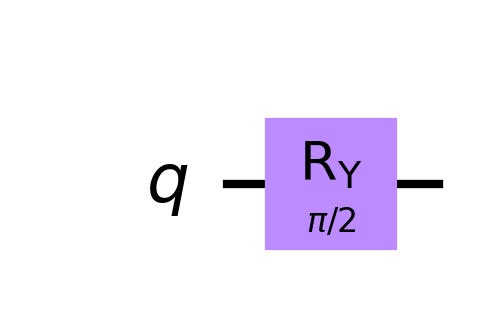
\includegraphics[width=0.65\linewidth]{figures/DarstellungGatter/ry_gatter_circuit.png}
        \subcaption{Schaltkreis mit \textit{RY}-Gatter}
        \label{fig:circuit-ry}
    \end{subfigure}\hfill
    \begin{subfigure}{0.45\textwidth}
        \centering
        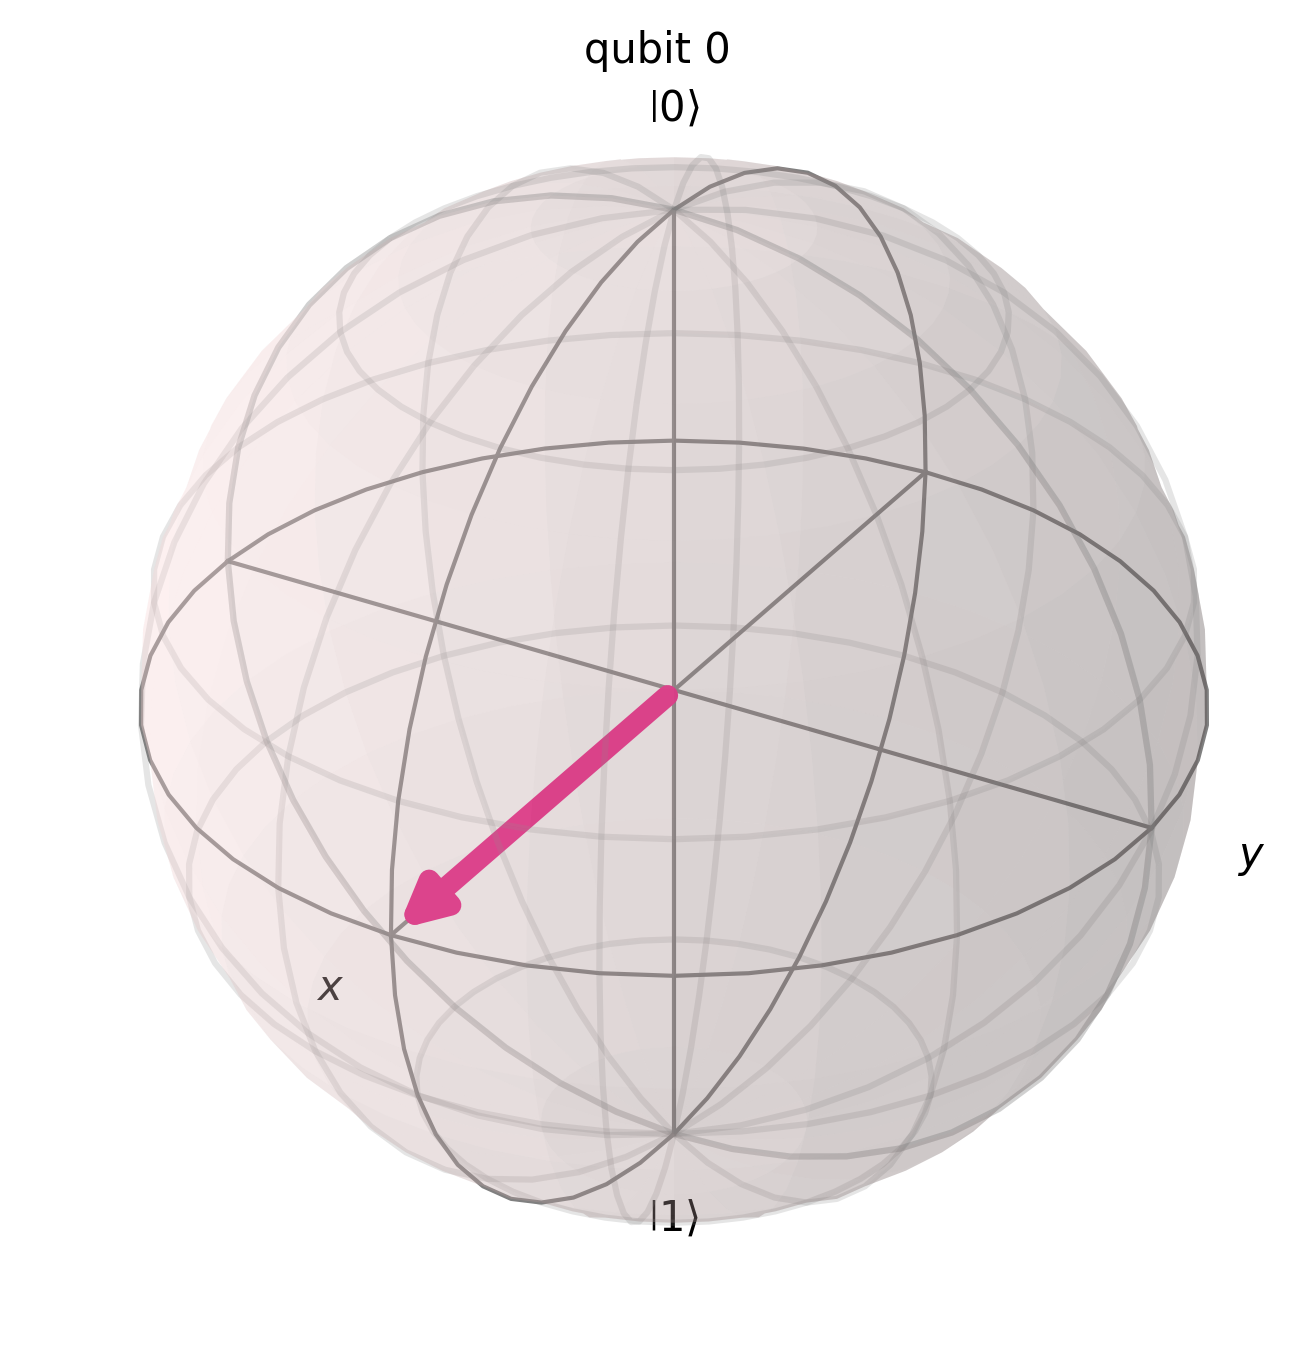
\includegraphics[width=0.65\linewidth]{figures/DarstellungGatter/ry_gatter_bloch.png}
        \subcaption{Zustand auf der Bloch-Sphäre}
        \label{fig:bloch-ry}
    \end{subfigure}
    \caption{Wirkung des \textit{RY}-Gatters für $\theta = \tfrac{\pi}{2}$}
    \label{fig:ry-gatter}
\end{figure}

\paragraph*{CNOT-Gatter}\mbox{}\\
Das \textit{CNOT-Gatter} (auch \textit{CX-Gatter}) ist das wichtigste
Zweiqubit-Gatter. Es wirkt auf ein \textit{Kontrollqubit} und ein
\textit{Zielqubit}. Befindet sich das Kontrollqubit im Zustand $\ket{1}$, wird auf
das Zielqubit eine $\mathbf{X}$-Operation angewendet, andernfalls bleibt das
Zielqubit unverändert. In der Zweiqubit-Basis
$\{\ket{00}, \ket{01}, \ket{10}, \ket{11}\}$ lautet die Matrixdarstellung
\begin{equation}
    \mathbf{CX} =
    \begin{pmatrix}
        1 & 0 & 0 & 0 \\
        0 & 1 & 0 & 0 \\
        0 & 0 & 0 & 1 \\
        0 & 0 & 1 & 0
    \end{pmatrix}.
\end{equation}
Die Wirkung auf die Basiszustände ergibt sich entsprechend zu
\begin{equation}
    \mathbf{CX}\ket{00} = \ket{00}, \quad
    \mathbf{CX}\ket{01} = \ket{01}, \quad
    \mathbf{CX}\ket{10} = \ket{11}, \quad
    \mathbf{CX}\ket{11} = \ket{10}.
\end{equation}
Wird das Gatter auf einen Basiszustand angewendet, entsteht dabei stets wieder ein
Produktzustand. Die besondere Bedeutung des CNOT-Gatters liegt darin, dass es aus einer
Superposition des Kontrollqubits Verschränkung erzeugt.
\begin{equation}
    \mathbf{CX}_{12}\,\mathbf{H}_1\ket{00}
    = \mathbf{CX}_{12}\,\frac{1}{\sqrt{2}}\bigl(\ket{00} + \ket{10}\bigr)
    = \frac{1}{\sqrt{2}}\bigl(\ket{00} + \ket{11}\bigr).
\end{equation}
Das Hadamard-Gatter versetzt zunächst das erste Qubit in eine Superposition (siehe
Abbildung~\ref{fig:circuit-cnot}). Das CNOT-Gatter wirkt anschließend auf beide
Anteile zugleich. Der Anteil $\ket{00}$ bleibt unverändert, im Anteil $\ket{10}$
wird das Zielqubit umgeklappt. Im Ergebnis liefern beide Qubits bei einer Messung
stets dasselbe Resultat, und der Zustand lässt sich nicht mehr als Tensorprodukt
einzelner Qubitzustände schreiben.

Anders als bei den bisher betrachteten Gattern lässt sich das Ergebnis nicht mehr
auf der Bloch-Sphäre darstellen. Diese beschreibt jeweils den Zustand eines
einzelnen Qubits, ein verschränkter Zustand ist jedoch nur als Ganzes definiert.
Betrachtet man eines der beiden Qubits für sich, so liefert es in jeder
Messrichtung beide Ergebnisse mit gleicher Wahrscheinlichkeit. Die eigentliche
Information liegt nicht in den einzelnen Qubits, sondern in ihrer Korrelation und
entzieht sich damit einer getrennten Darstellung.

\begin{figure}[htbp]
    \centering
    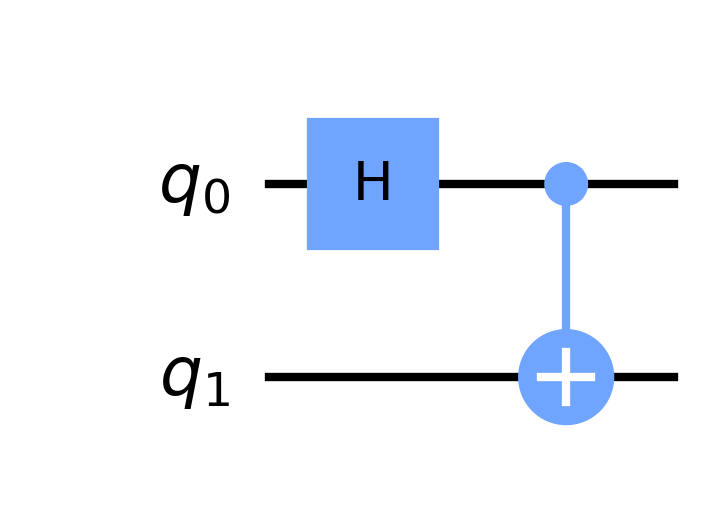
\includegraphics[width=0.3\textwidth]{figures/DarstellungGatter/cnot_gatter_circuit.png}
    \caption{Schaltkreis mit \textit{H}- und \textit{CNOT}-Gatter}
    \label{fig:circuit-cnot}
\end{figure}

% ----------------------------------------------------------------
\newpage

\section{Observablenberechnung}
\label{sec:observablen}

Als \textit{Observable} wird in der Quantenmechanik eine messbare physikalische
Größe bezeichnet, die durch einen hermiteschen Operator repräsentiert
wird~\cite{nielsen2010chuang}. Ein Operator heißt \textit{hermitesch}, wenn er mit
seinem adjungierten Operator übereinstimmt, also $O = O^{\dagger}$ gilt, wobei
$O^{\dagger}$ die konjugiert transponierte Matrix bezeichnet. Diese Eigenschaft
stellt sicher, dass alle Eigenwerte reell sind, was Voraussetzung dafür ist, dass
sie als physikalische Messwerte interpretiert werden können. Welcher Eigenwert bei
einer einzelnen Messung auftritt, ist im Allgemeinen nicht vorhersagbar, sondern
folgt einer durch den Quantenzustand festgelegten Wahrscheinlichkeitsverteilung.

Da einzelne Messungen zufällig ausfallen, ist im Quantencomputing weniger das
Einzelergebnis als vielmehr der \textit{Erwartungswert} einer Observablen $O$
bezüglich eines Zustands $\ket{\psi}$ von Interesse. Dieser ist definiert als
\[
    \expval{O} = \bra{\psi} O \ket{\psi}
\]
und beschreibt den statistischen Mittelwert der Messergebnisse über viele
Wiederholungen. Seine Berechnung beziehungsweise Schätzung bildet die Grundlage zahlreicher
Quantenalgorithmen.

Für die konkrete Darstellung von Observablen werden üblicherweise die
Pauli-Operatoren $I$, $X$, $Y$ und $Z$ herangezogen. Diese bilden mit reellen
Koeffizienten eine Basis des Raums der hermiteschen $2 \times 2$-Matrizen, sodass
sich jede Observable eines einzelnen Qubits als Linearkombination dieser vier
Operatoren schreiben lässt~\cite{nielsen2010chuang}. Für Systeme mehrerer Qubits
werden Observablen entsprechend als Linearkombination von Tensorprodukten dieser
Operatoren ausgedrückt, die als \enquote{Pauli-Strings} bezeichnet werden.
\newpage